\documentclass{beamer}
\usetheme{CambridgeUS}
\usepackage[T1]{fontenc}
\usepackage[utf8]{inputenc}
\usepackage[english]{babel}
\usepackage{comment}
\usepackage{booktabs}
\usepackage{multirow}
\usepackage{graphicx}
\usepackage{verbatim}
\usepackage{lmodern}
\usepackage{textcomp}

\title[Load testing of distributed applications]{Load testing of distributed applications:\\the Signal case study}
\titlegraphic{
    \centering
    
\includegraphics[width=1.5cm]{img/logo_unipd}
}
\author[M.~Marchiori]{Master candidate: Matteo Marchiori\\Supervisor: Tullio Vardanega}
\institute[University of Padua]{University of Padua\\Department of Mathematics ``Tullio Levi-Civita''\\Master degree in Computer Science\\Final exam}
\date{15-12-2021}

\begin{document}

\begin{frame}
    \maketitle
\end{frame}

\begin{frame}{Contents}
    \tableofcontents
\end{frame}

\section{Problem statement}

\begin{frame}{Aim of the work}
    \begin{block}{}
        \begin{itemize}
            \item Resources to study cloud-native execution behavior
            \item Load testing as a tool
            \item 
\includegraphics[width=.03\textwidth]{img/signal} as a case study application
        \end{itemize}
    \end{block}
    \centering
    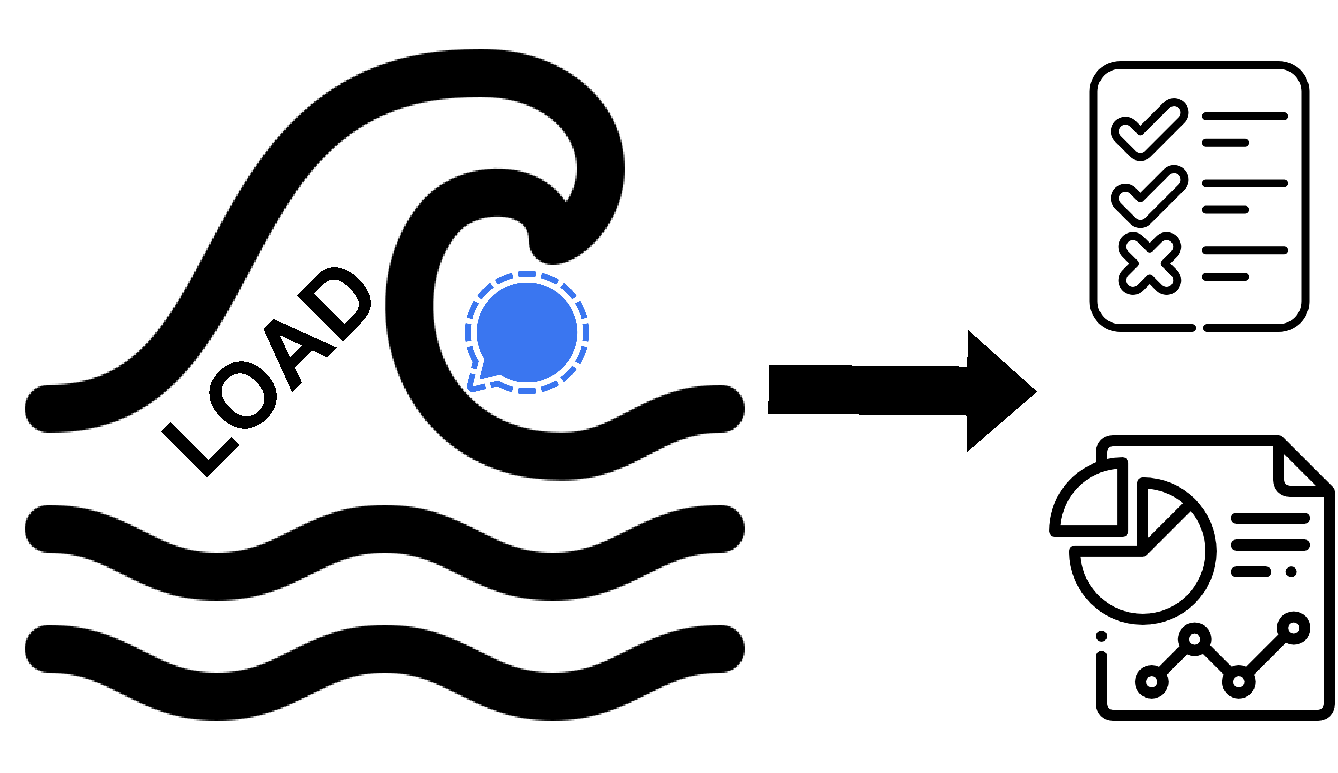
\includegraphics[width=.75\textwidth]{img/wave}
\end{frame}

\subsection{Scalability}
\begin{frame}{What is scalability}
    \centering
    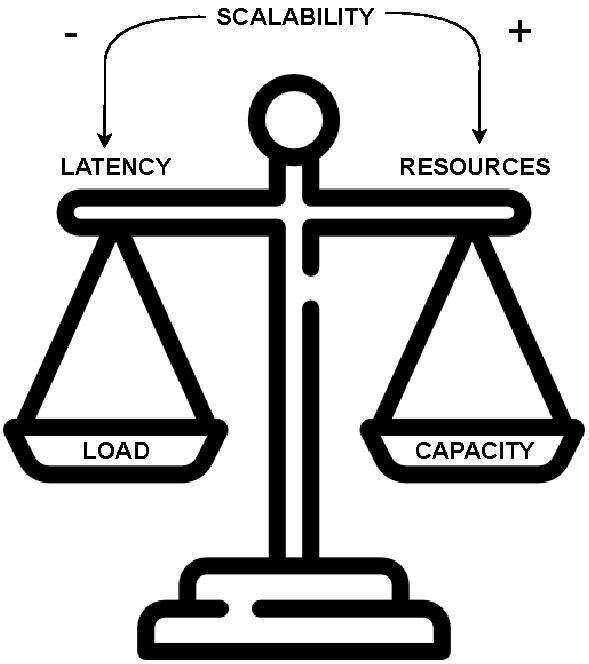
\includegraphics[width=.5\textwidth]{img/balance}
\end{frame}

\begin{frame}{Scalability dimensions}
    \begin{columns}
        \begin{column}{.3\textwidth}
            \centering
            Functional decomposition
        \end{column}
        \begin{column}{.3\textwidth}
            \centering
            Horizontal replication
        \end{column}
        \begin{column}{.3\textwidth}
            \centering
            Data partitioning
        \end{column}
    \end{columns}
    \vfill
    \centering
    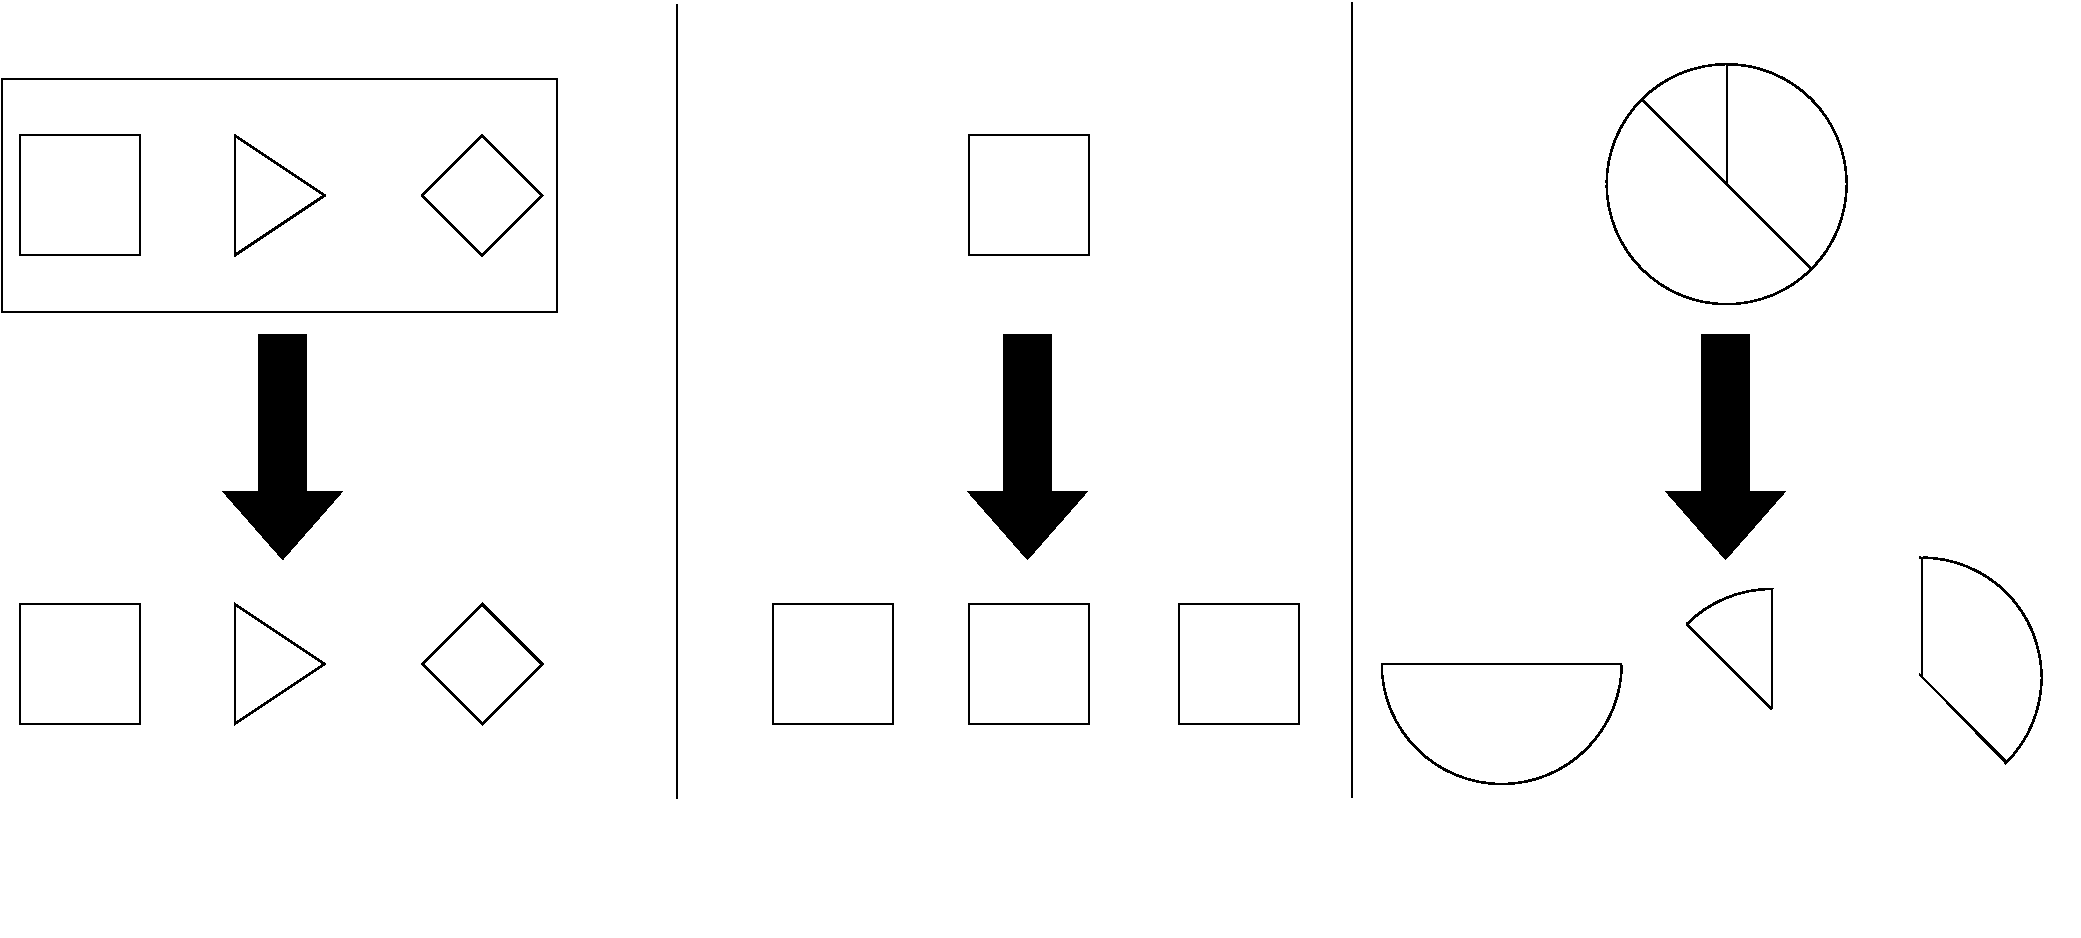
\includegraphics[width=\textwidth]{img/dimensions}
\end{frame}

\section{Approach}

\subsection{Signal architecture and experiments}

\begin{frame}{Signal architectures' comparison}
    \begin{columns}[t]
        \begin{column}{.4\textwidth}
            Signal 4.97
            \begin{itemize}
                \item Outage case study - January 2021
                \item More self-contained components
            \end{itemize}
        \end{column}
        \begin{column}{.4\textwidth}
            Signal 6.13
            \begin{itemize}
                \item Most recent version - July 2021
                \item More AWS components
            \end{itemize}
        \end{column}
    \end{columns}

    \vfill

    \centering
    
\includegraphics[width=.7\textwidth]{img/postgresql-dynamodb}
\end{frame}

\begin{frame}{Server general architecture}
    \centering
    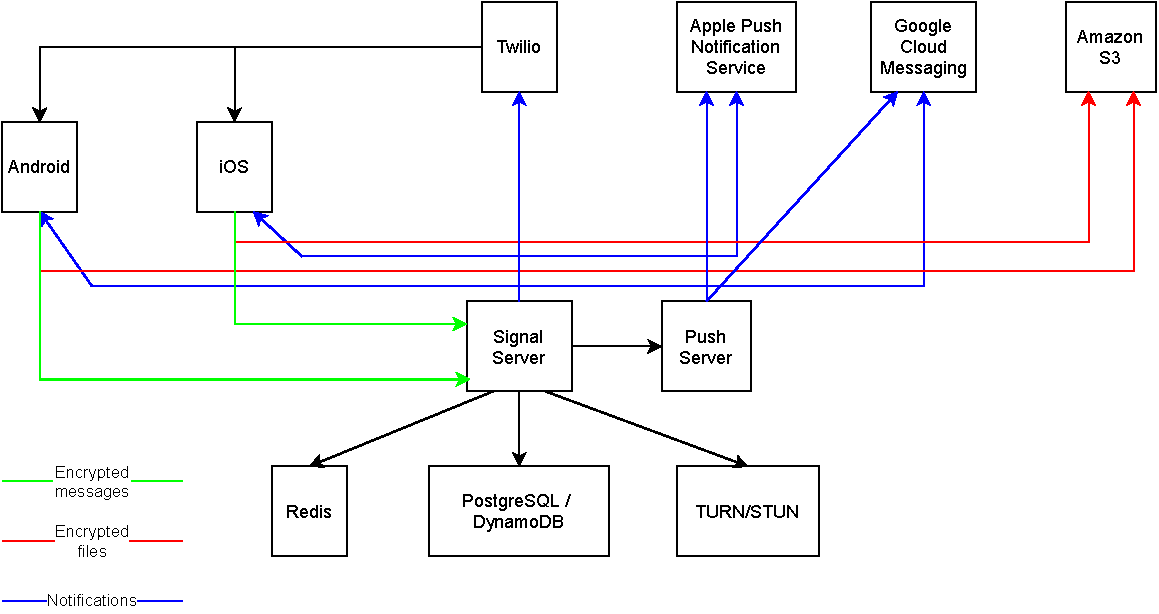
\includegraphics[width=.9\textwidth]{img/Architecture}
    https://sorincocorada.ro/signal-messanger-architecture/
\end{frame}

\begin{frame}{Involved components and calls order}
    \centering
    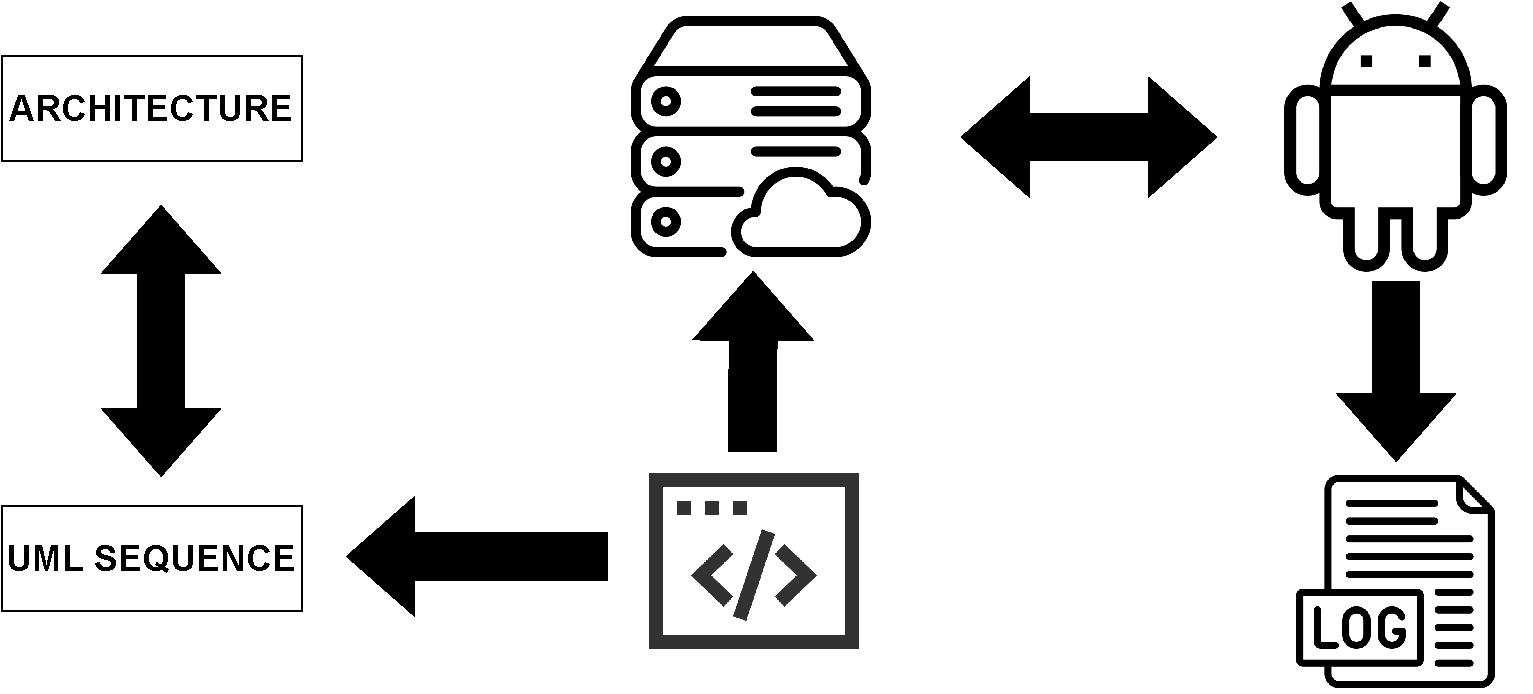
\includegraphics[width=\textwidth]{img/components}
\end{frame}

\begin{frame}{Kind of experiments}
    Steady load
    \begin{block}{}
        \centering
        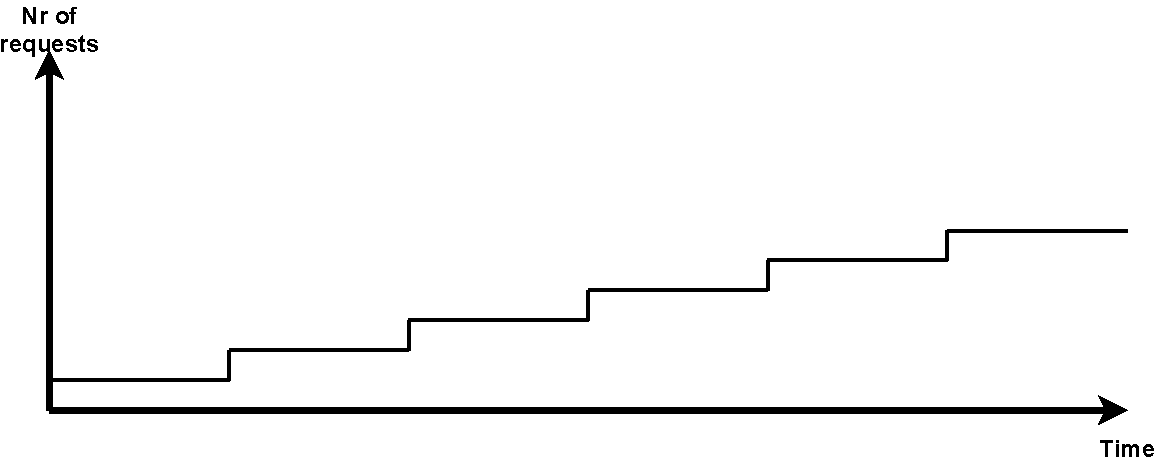
\includegraphics[width=.6\textwidth]{img/steady}
    \end{block}
    Peak load
    \begin{block}{}
        \centering
        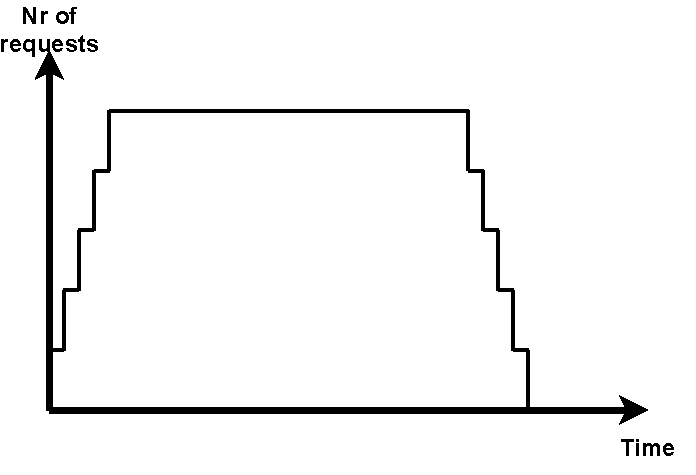
\includegraphics[width=.35\textwidth]{img/peak}
    \end{block}
\end{frame}

\begin{frame}{Tools}
    \centering
    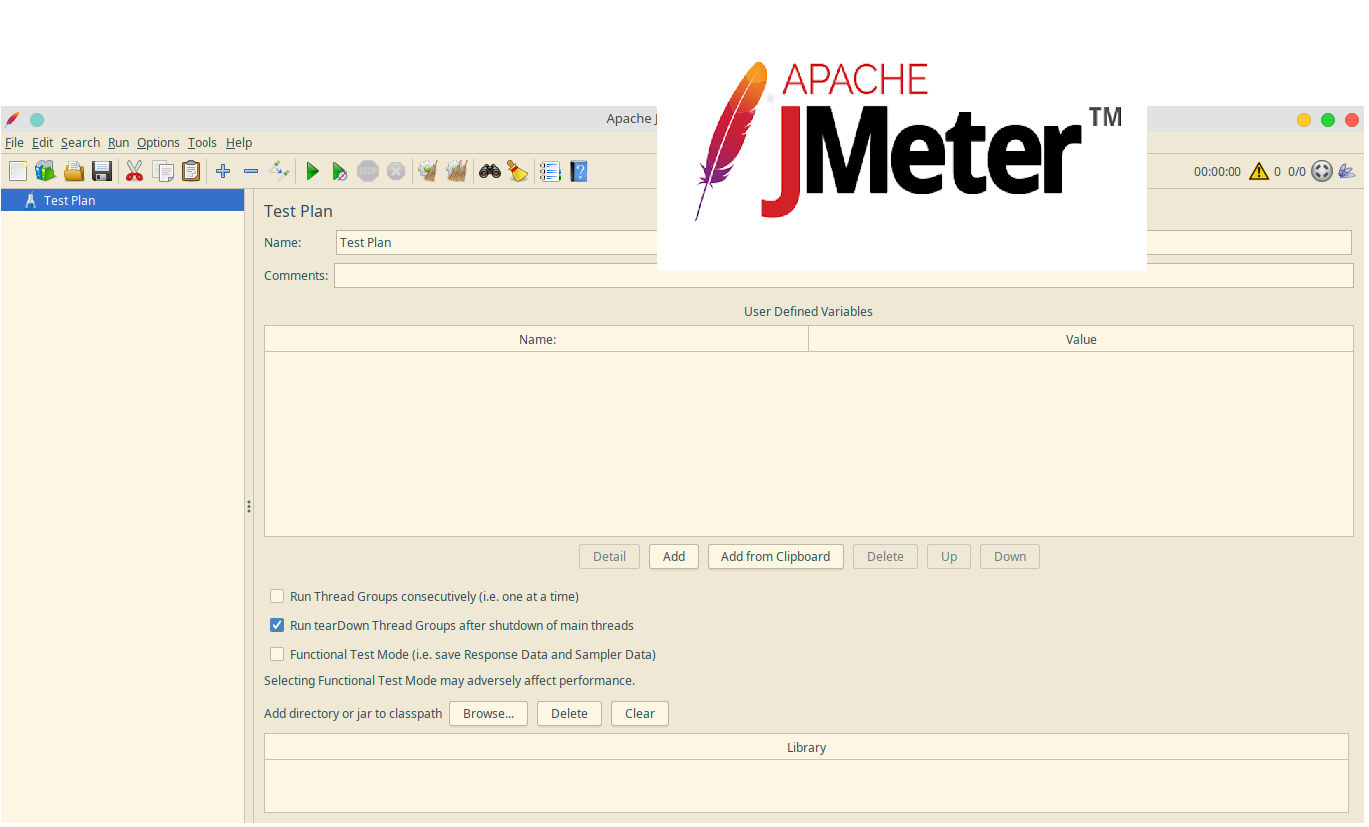
\includegraphics[width=.75\textwidth]{img/jmeter}
\end{frame}

\section{Results}

\subsection{Metrics}
\begin{frame}{Request metrics}
    \begin{itemize}
        \item average response time (ms)
        \item median response time (ms)
        \item 90th, 95th and 99th percentile response time (ms)
    \end{itemize}

    \begin{table}[H]
    \resizebox{\textwidth}{!}{%
    \begin{tabular}{@{}lllllllllll@{}}
    \toprule
    \multicolumn{1}{c}{\multirow{2}{*}{\textbf{Request}}} & \multicolumn{1}{c}{\multirow{2}{*}{\textbf{\#Samples}}} & \multicolumn{7}{c}{\textbf{Response times (ms)}} & \multicolumn{2}{c}{\textbf{Network (KB/s)}} \\ \cmidrule(l){3-11} 
    \multicolumn{1}{c}{} & \multicolumn{1}{c}{} & \multicolumn{1}{c}{Average} & \multicolumn{1}{c}{Min} & \multicolumn{1}{c}{Max} & \multicolumn{1}{c}{Median} & \multicolumn{1}{c}{90th pct} & \multicolumn{1}{c}{95th pct} & \multicolumn{1}{c}{99th pct} & \multicolumn{1}{c}{Received} & \multicolumn{1}{c}{Sent} \\ \midrule
    GET /v1/profile & 48665 & 2083.32 & 23 & 130681 & 3032.00 & 3785.00 & 9200.95 & 35696.04 & 63.51 & 36.36 \\
    GET /v2/keys/+391234567890/* & 48442 & 1920.06 & 17 & 129352 & 2989.00 & 3691.00 & 6656.70 & 10982.99 & 37.58 & 9.93 \\
    PUT /v1/messages & 48300 & 2227.99 & 20 & 130654 & 3063.50 & 6985.40 & 9446.95 & 38666.65 & 19.67 & 31.07
    \end{tabular}%
    }
    \end{table}
\end{frame}

\begin{frame}{Performance metrics}
    \begin{itemize}
        \item percentage of CPU used per second
        \item percentage of memory used per second
        \item network I/O (B/s)
    \end{itemize}

    \vfill
    \centering
    
\includegraphics[width=.7\textwidth]{img/resources}
\end{frame}

\begin{frame}{Environment characteristics}
    \centering
    
\includegraphics[width=.5\textwidth]{img/clientserver}
    
    \begin{columns}[t]
        \begin{column}{.4\textwidth}
            \begin{itemize}
                \item Intel(R) Core(TM) i3-4005U CPU @ $1.70$GHz
                \item $4$GB of RAM
                \item Ubuntu 21.04
                \item Apache JMeter 5.4.1
            \end{itemize}
        \end{column}
        \begin{column}{.4\textwidth}
            \begin{itemize}
                \item $2$ vCPUs of burstable type
                \item $1$ GB of RAM
                \item Ubuntu 20.04.3 LTS
                \item Dropwizard 2.0.13 / 2.0.22
                \item Redis server v=5.0.7
                \item PostgreSQL 12.9
                \item Nginx 1.18.0
            \end{itemize}
        \end{column}
    \end{columns}
\end{frame}

\subsection{Experimental results}

\begin{frame}{Account creation - steady load}
    \centering
    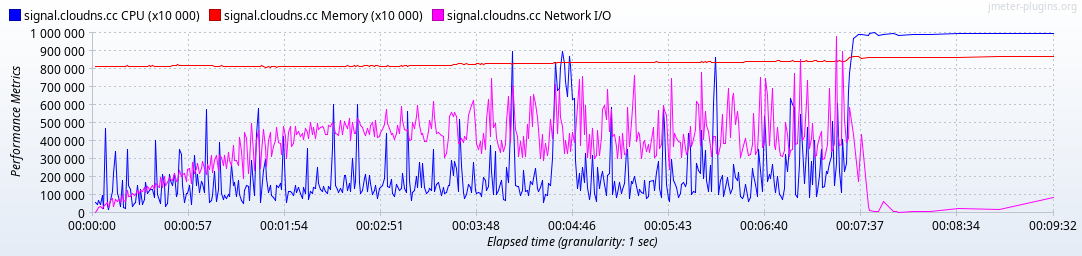
\includegraphics[width=\textwidth]{img/4.97-steady-create}

    \vfill

    \centering
    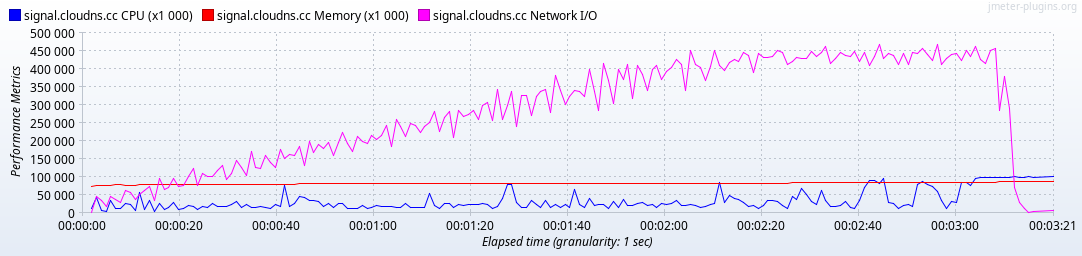
\includegraphics[width=\textwidth]{img/6.13-steady-create}
\end{frame}

\begin{frame}{Message sending - steady load}
    \centering
    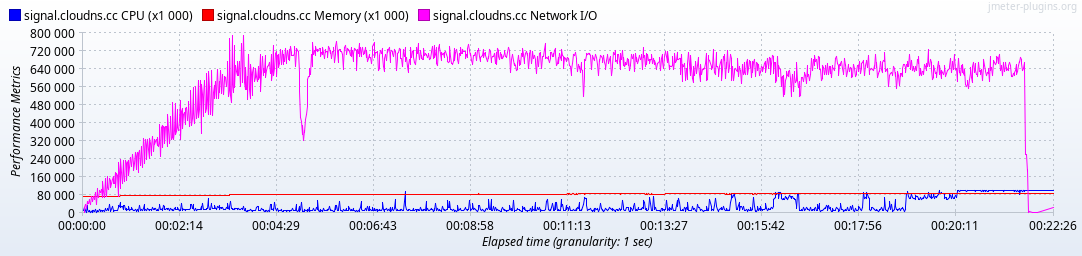
\includegraphics[width=\textwidth]{img/4.97-steady-message}

    \vfill

    \centering
    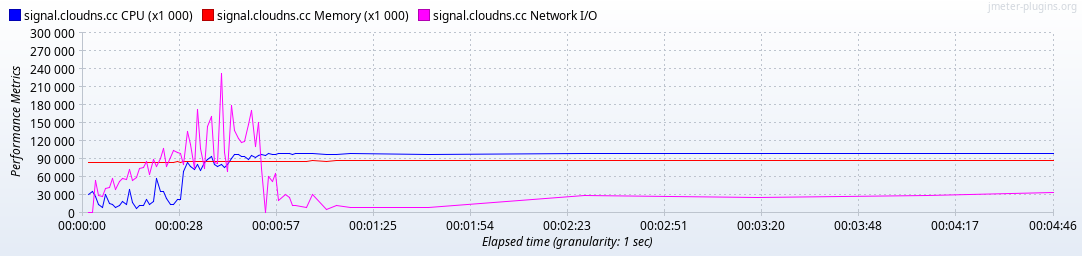
\includegraphics[width=\textwidth]{img/6.13-steady-message}
\end{frame}

\begin{frame}{Account creation - peak load}
    \centering
    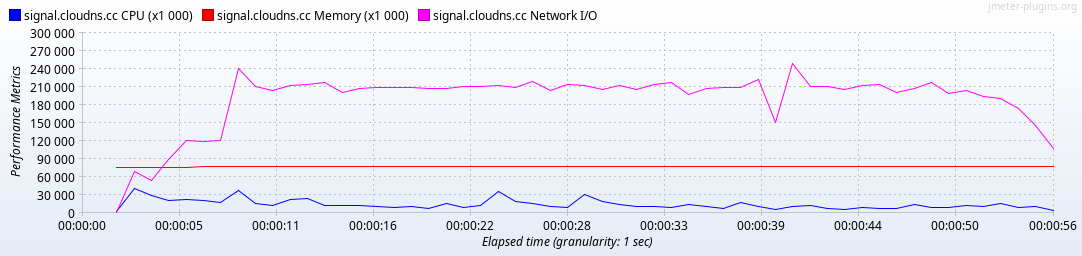
\includegraphics[width=\textwidth]{img/4.97-peak-create}

    \vfill

    \centering
    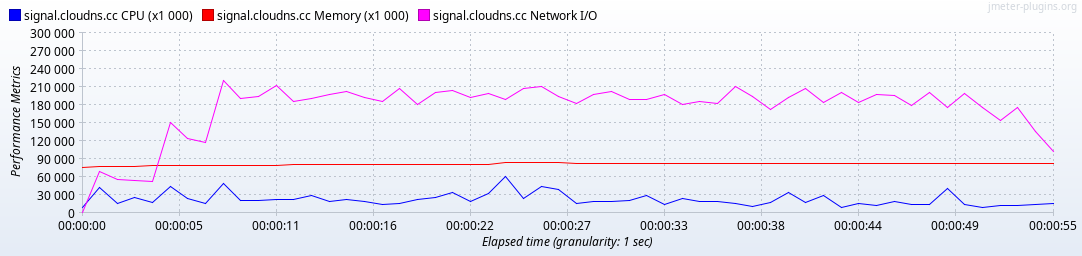
\includegraphics[width=\textwidth]{img/6.13-peak-create}
\end{frame}

\begin{frame}{Message sending - peak load}
    \centering
    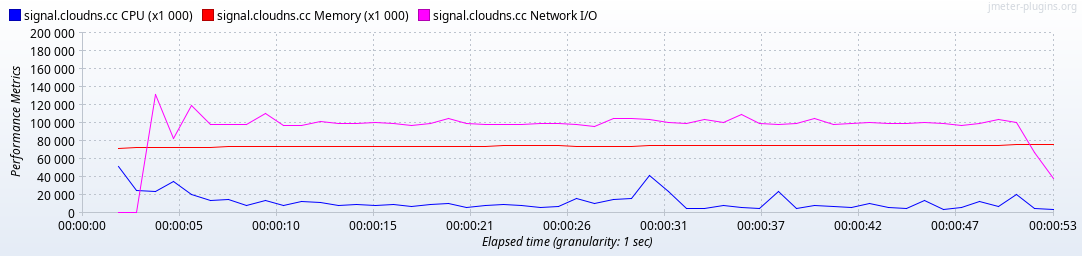
\includegraphics[width=\textwidth]{img/4.97-peak-message}

    \vfill

    \centering
    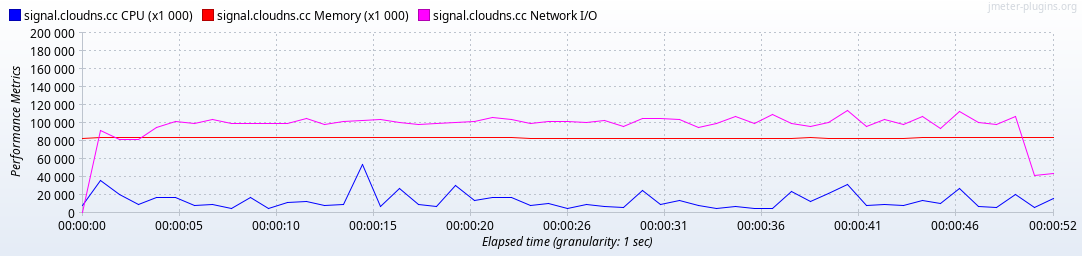
\includegraphics[width=\textwidth]{img/6.13-peak-message}
\end{frame}

\section{Conclusions}

\begin{frame}{Observations and outlook}
    \begin{block}{}
        \begin{itemize}
            \item Real examples \(\rightarrow\) load experiments
            \item Steady load \(\rightarrow\) Signal 4.97 wins
            \item Peak load \(\rightarrow\) Signal 6.13 wins
            \item Test of similar kind of applications
            \item Test with other load on components (not only black box tests)
            \item Expand the tests to other Signal functionalities (video/audio calls)
            \item Test in real world environment
        \end{itemize}
    \end{block}
\end{frame}

\end{document}